\documentclass[12pt]{exam}
\usepackage[margin=1cm,papersize={8.5in,17in}]{geometry}
\usepackage{enumitem}
\usepackage{tikz}
\usepackage{circuitikz}
\usepackage{newtxtext,newtxmath}
\usepackage{siunitx}
\usepackage{multicol}
\usepackage{bm}

\usetikzlibrary{patterns}

\newcommand{\pic}[2]{\includegraphics[width=#1\textwidth]{#2}}
\renewcommand{\choicelabel}{(\thechoice)}
\sisetup{
  inter-unit-product =\ensuremath{\cdot{}},
  per-mode=symbol
}
\tikzset{
  >=latex
}
\pagestyle{empty}

\renewcommand{\choiceshook}{
  \setlength{\leftmargin}{25pt}
  \setlength{\itemsep}{2.5pt}%.9\baselineskip}
  \setlength{\topsep}{0pt}
  %\setlength\partopsep{100pt} 
  \setlength\parsep{0pt}
}

\begin{document}
\begin{center}
  \textbf{PHYSICS C: ELECTRICITY AND MAGNETISM\\
    Section I\\
    Time--45 minutes\\
    35 Questions
  }
\end{center}
\raggedcolumns

\textbf{Directions:} Each of the questions or incomplete statements below is
followed by five suggested answers or completions. Select the one that is best
in each case and place the letter of your choice in the corresponding box on
the student answer sheet.

\begin{questions}
  \question Two negative point charges are a distance $x$ apart and have
  potential energy $U$. If the distance between the point charges increases to
  $3x$, what is their new potential energy?
  \begin{choices}
    \choice $9U$
    \choice $3U$
    \choice $U$
    \choice $U/3$
    \choice $U/9$
  \end{choices}

  \begin{center}
    \pic{.3}{rod1}
  \end{center}
  \question An electric field is produced by the very long, uniformly charged
  rod drawn above. If the strength of the electric field is $E_1$ at a distance
  $r_1$ from the axis of the rod, at what distance from the axis is
  the field strength $\dfrac{E_1}4$?
  \begin{choices}
    \choice $\dfrac{r_1}4$
    \choice  $\dfrac{r_1}2$
    \choice $2r_1$
    \choice $4r_1$
    \choice $16r_1$
  \end{choices}
  
  \fullwidth{
    \textbf{Question \ref{sphere1}--\ref{sphere2}}
    \begin{center}
      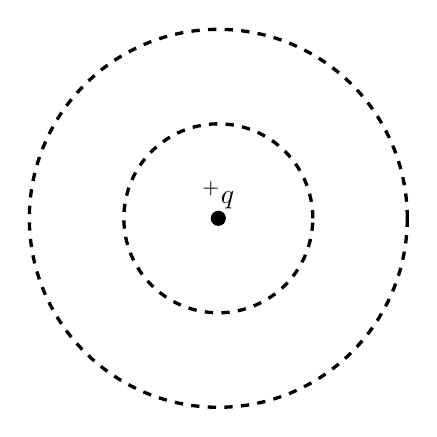
\begin{tikzpicture}[scale=1.2]
        \fill(0,0) circle(.08) node[above]{$^+q$}; 
        \draw[very thick,dashed](0,0) circle(1);
        \draw[very thick,dashed](0,0) circle(2);
      \end{tikzpicture}
    \end{center}
    Two concentric spherical surfaces are drawn around an isolated positive
    charge $+q$ located at their center, as shown above. The inner surface has
    a radius that is $1/2$ that of the outer surface.
  }

  \question If the total electric flux passing through the inner surface is
  $\phi$, what is the total electric flux passing through the outer surface?
  \begin{choices}
    \choice $\phi/4$
    \choice $\phi/2$
    \choice $\phi$
    \choice $2\phi$
    \choice $4\phi$
  \end{choices}
  \label{sphere1}
  
  \question If the electric field strength at the inner surface is $E$, what is
  the electric field strength at the outer surface?
  \begin{choices}
    \choice $E/4$
    \choice $E/2$
    \choice $E$
    \choice $2E$
    \choice $4E$
  \end{choices}
  \label{sphere2}
  \newpage
  
  \begin{center}
    \pic{.3}{2spheres}
  \end{center}
  \question Sphere $X$ of mass $M$ and charge $+q$ hangs from a string as shown
  above. Sphere $Y$ has an equal charge $+q$ and is fixed in place a distance
  $d$ directly below sphere $X$. If sphere $X$ is in equilibrium, the tension
  in the string is most nearly
  \begin{choices}
    \choice $Mg$
    \choice $Mg+\dfrac{kq}d$
    \choice $Mg-\dfrac{kq}d$
    \choice $Mg+\dfrac{kq^2}{d^2}$
    \choice $Mg-\dfrac{kq^2}{d^2}$
  \end{choices}

  \begin{center}
    \pic{.22}{tetrahedral}
  \end{center}
  \question A charge $+q$ is placed at the center of a tetrahedron whose faces
  are all equilateral triangles, as shown above. What is the flux of the
  electric field through one face of the tetrahedron?
  \begin{choices}
    \choice 0
    \choice $\dfrac{q}{\epsilon_0}$
    \choice $\dfrac{q}{4\epsilon_0}$
    \choice $4\epsilon_0q$
    \choice The flux through one face cannot be determined from the information
    given.
  \end{choices}

  \begin{center}
    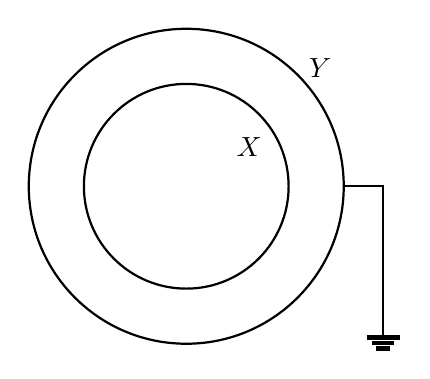
\begin{tikzpicture}
      \begin{scope}[thick]
        \draw(0,0) circle(1.3);
        \draw(0,0) circle(2);
        \draw(2,0)--(2.5,0)--(2.5,-1.5) node[ground]{};
      \end{scope}
      \node at (.8,.5) {$X$};
      \node at (1.7,1.5) {$Y$};
    \end{tikzpicture}
  \end{center}
  \question Two concentric metal spheres $X$ and $Y$ are shown above. $X$
  carries a positive charge, and $Y$ is connected to ground. True statements
  include which of the following?
  \begin{enumerate}[topsep=0pt,itemsep=2pt]
  \item[I.] The electric field inside $X$ is zero.
  \item[II.] The electric field outside $Y$ is zero.
  \item[III.] The charge density on both spheres is the same.
  \end{enumerate}
  \begin{choices}
    \choice I only
    \choice III only
    \choice I and II only
    \choice II and III only
    \choice I, II, and III
  \end{choices}
  \newpage

  \begin{center}
    \pic{.3}{cup}
  \end{center}
  \question A small positively charged sphere is lowered by a nonconducting
  thread into a grounded metal cup without touching the inside surface of the
  cup, as shown above. The grounding wire attached to the outside surface is
  disconnected and the charged sphere is then removed from the cup. Which of
  the following best describes the subsequent distribution of excess charge on
  the surface of the cup?
  \begin{choices}
    \choice Negative charge resides on the inside surface, and no charge
    resides on the outside surface.
    \choice Negative charge resides on the outside surface, and no charge
    resides on the inside surface.
    \choice Positive charge resides on the inside surface, and no charge
    resides on the outside surface.
    \choice Positive charge resides on the outside surface, and no charge
    resides on the inside surface.
    \choice Negative charge resides on the inside surface, and positive charge
    resides on the outside surface.
  \end{choices}
  \vspace{.7in}

  \begin{center}
    \pic{.35}{rc1}
  \end{center}
  \question The capacitor $C$ in the circuit shown above is initially
  uncharged. The switch $S$ is then closed. Which of the following best
  represents the voltage $V_R$ across the resistor $R$ as a function of time
  $t$?
  
  \begin{oneparchoices}
    \choice
    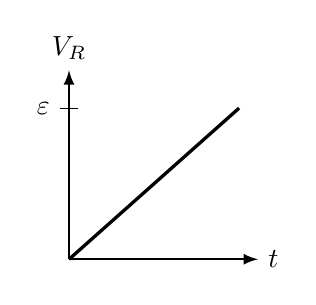
\begin{tikzpicture}[scale=1.2]
      \draw[thick,->](0,0)--(2,0)node[right]{$t$};
      \draw[thick,->](0,0)--(0,2)node[above]{$V_R$};
      \draw[very thick](0,0)--(1.8,1.6);
      \draw(.1,1.6)--(-.1,1.6) node[left]{$\varepsilon$};
    \end{tikzpicture}

    \choice
    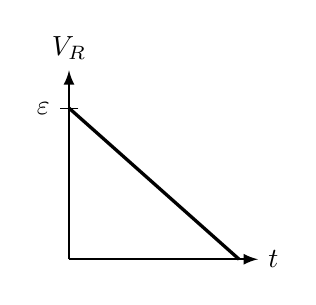
\begin{tikzpicture}[scale=1.2]
      \draw[thick,->](0,0)--(2,0)node[right]{$t$};
      \draw[thick,->](0,0)--(0,2)node[above]{$V_R$};
      \draw[very thick](0,1.6)--(1.8,0);
      \draw(.1,1.6)--(-.1,1.6) node[left]{$\varepsilon$};
      %\draw[thick,domain=0:1.7] plot(\x,{-\x*\x*.43+1.6});
    \end{tikzpicture}

    \choice
    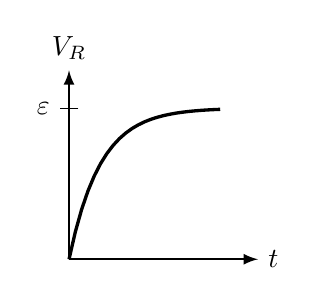
\begin{tikzpicture}[scale=1.2]
      \draw[thick,->](0,0)--(2,0)node[right]{$t$};
      \draw[thick,->](0,0)--(0,2)node[above]{$V_R$};
      \draw(.1,1.6)--(-.1,1.6) node[left]{$\varepsilon$};
      \draw[very thick,domain=0:1.6] plot(\x,{1.6*(1-exp(-3*\x))});
    \end{tikzpicture}

    \choice
    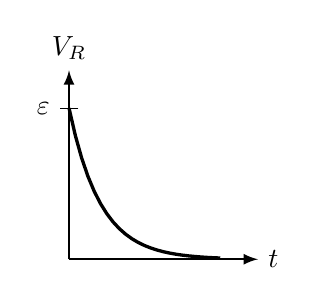
\begin{tikzpicture}[scale=1.2]
      \draw[thick,->](0,0)--(2,0)node[right]{$t$};
      \draw[thick,->](0,0)--(0,2)node[above]{$V_R$};
      \draw(.1,1.6)--(-.1,1.6) node[left]{$\varepsilon$};
      \draw[very thick,domain=0:1.6] plot(\x,{1.6*exp(-3*\x))});
    \end{tikzpicture}

    \choice
    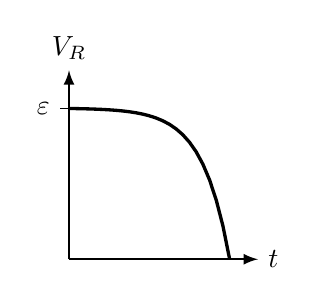
\begin{tikzpicture}[scale=1.2]
      \draw[thick,->](0,0)--(2,0)node[right]{$t$};
      \draw[thick,->](0,0)--(0,2)node[above]{$V_R$};
      \draw(.1,1.6)--(-.1,1.6) node[left]{$\varepsilon$};
      \draw[very thick,domain=0:1.7] plot(\x,{1.6*(1-exp(3.5*(\x-1.7)))});
    \end{tikzpicture}
  \end{oneparchoices}
  
%  \question In an experiment with a simple pendulum, measurements of the period
%  $T$ of the pendulum are made for different values of its length $L$.
%  When plotted on a graph, which of the following should result in a
%  straight-line fit of the data?
%  \begin{choices}
%    \choice $\sqrt{T}$ versus $L$
%    \choice $T$ versus $L$
%    \choice $T$ versus $L^2$
%    \choice $T^2$ versus $L$
%    \choice $T^2$ versus $L^2$
%  \end{choices}
%
%  \begin{center}
%    \vspace{-.3in} 
%    \pic{.15}{comet}
%  \end{center}
%  \question A comet moves in the Sun's gravitational field, following the path
%  shown above. What happens to its angular momentum as it moves from point $X$
%  to point $Y$?
%  \begin{choices}
%    \choice It increases steadily.
%    \choice It remains constant.
%    \choice It decreases steadily.
%    \choice It increases as it approaches the Sun and decreases as it moves
%    away from the Sun.
%    \choice It decreases as it approaches the Sun and increases as it moves
%    away from the Sun.
%  \end{choices}
%  \vspace{.7in}
%
%  \question Satellite $X$ moves around Earth in a circular orbit of radius $R$.
%  Satellite $Y$ is also in a circular orbit around Earth, and it completes one
%  orbit for every eight orbits completed by satellite $X$. What is the
%  orbital radius of satellite $Y$?
%  \begin{choices}
%    \choice $R/4$
%    \choice $R/2$
%    \choice $2R$
%    \choice $4R$
%    \choice $8R$
%  \end{choices}
%
%  \question A newly discovered planet is found to have twice the radius and five
%  times the mass of Earth. If the acceleration of gravity at the surface of
%  Earth is $g$, the acceleration of gravity at the surface of the new planet is
%
%  \begin{choices}
%    \choice $\dfrac{2g}5$
%    \choice $\dfrac{4g}5$
%    \choice $g$
%    \choice $\dfrac{5g}4$
%    \choice $\dfrac{5g}2$
%  \end{choices}
%
%  \fullwidth{
%    \textbf{Questions \ref{toycar1}--\ref{toycar2}}
%    
%    A toy car of mass 6 kg, moving in a straight path, experiences a net force
%    given by the function $F=-3t$. At time $t=0$, the car has a velocity of
%    \SI{4}{\metre\per\second} in the positive direction and is located
%    $+8$ \si{\metre} from the origin.
%  }
%  
%  \question The car will come instantaneously to rest at time $t$ equal to
%  \label{toycar1}
%  \begin{choices}
%    \choice$\dfrac23$ \si\second
%    \choice$\sqrt{\dfrac43}$ \si\second
%    \choice$\sqrt{\dfrac83}$ \si\second
%    \choice$\sqrt8$ \si\second
%    \choice\SI{4}{\second}
%  \end{choices}
%
%
%  \question Which of the following best shows a graph of position $d$ versus
%  time $t$ for the car?
%  
%  \begin{oneparchoices}
%    \choice
%    \begin{tikzpicture}[scale=1.2]
%      \draw[thick,->](-.2,0)--(2,0)  node[right]{$t$};
%      \draw[thick,->](0,-.2)--(0,1.5)node[above]{$d$};
%      \draw[thick](0,1.2)--(1.8,-.2);
%    \end{tikzpicture}
%
%    \choice
%    \begin{tikzpicture}[scale=1.2]
%      \draw[thick,->](-.2,0)--(2,0)  node[right]{$t$};
%      \draw[thick,->](0,-.75)--(0,1.25)node[above]{$d$};
%      \draw[thick] (0,.5)--(.5,.5) to [out=0,in=180](1.5,-.5)--(2,-.5);
%    \end{tikzpicture}
%
%    \choice
%    \begin{tikzpicture}[scale=1.2]
%      \draw[thick,->](-.2,0)--(2,0)  node[right]{$t$};
%      \draw[thick,->](0,-.2)--(0,1.5)node[above]{$d$};
%      \draw[thick,domain=0:1.8]plot(\x,{1.2*exp(-2*\x)});
%    \end{tikzpicture}
%    
%    \choice
%    \begin{tikzpicture}[scale=1.2]
%      \draw[thick,->](-.2,0)--(2,0)  node[right]{$t$};
%      \draw[thick,->](0,-.2)--(0,1.5)node[above]{$d$};
%      \draw[thick,domain=0:1.8]plot(\x,{-4*(.6*\x-.5)*(.6*\x-.5)+1});
%
%    \end{tikzpicture}
%
%    \choice
%    \begin{tikzpicture}[scale=1.2]
%      \draw[thick,->](-.2,0)--(2,0)  node[right]{$t$};
%      \draw[thick,->](0,-.2)--(0,1.5)node[above]{$d$};
%      \draw[thick,domain=0:1.6]plot(\x,{-(\x-.5)*(\x-.5)+1});
%    \end{tikzpicture}
%  \end{oneparchoices}
%  \label{toycar2}
%  
%  \fullwidth{
%    \textbf{Questions \ref{connect1}--\ref{connect2}}
%    \begin{center}
%      \pic{.3}{connected-mass}
%    \end{center}
%    A block of mass $M_1$ on a horizontal table is connected to a hanging block
%    of mass $M_2$ by a string that passes over a pulley, as shown above. The
%    acceleration of the blocks is $0.6g$. Assume that friction and the mass of
%    the string are negligible.
%  }
%
%  \question The tension $T$ in the string is \label{connect1}
%  \begin{choices}
%    \choice zero
%    \choice $0.4M_2g$
%    \choice $0.6M_2g$
%    \choice $1.0M_2g$
%    \choice $1.6M_2g$
%  \end{choices}
%  
%  \question The ratio of masses $M_2/M_1$ is  \label{connect2}
%  \begin{choices}
%    \choice 0.67
%    \choice 1.0
%    \choice 1.4
%    \choice 1.5
%    \choice 1.6
%  \end{choices}
%  
%  \fullwidth{
%    \textbf{Questions \ref{spring1}--\ref{spring2}}
%    \begin{center}
%      \pic{.28}{spring-mass}
%    \end{center}
%    \vspace{-.1in}In the system of two blocks and a spring shown above, blocks
%    1 and 2 are
%    connected by a string that passes over a pulley. The initially unstretched
%    spring connects block 1 to a rigid wall. Block 1 is released from rest,
%    initially slides to the right, and is eventually brought to rest by the
%    spring and by friction on the horizontal surface.
%  }
%
%  \question Which of the following is true of the energy of the system during
%  this process?
%  \begin{choices}
%    \choice The total mechanical energy of the system is conserved.
%    \choice The total mechanical energy of the system increases.
%    \choice The energy lost to friction is equal to the gain in the potential
%    energy of the spring.
%    \choice  The potential energy lost by block 2 is less in magnitude than the
%    potential energy gained by the spring.
%    \choice The potential energy lost by block 2 is greater in magnitude than
%    the potential energy gained by the spring.
%  \end{choices}
%  \label{spring1}
%  \vspace{.7in}
%
%  \question After block 1 comes to rest, the force exerted on it by the spring
%  must be equal in magnitude to
%  \begin{choices}
%    \choice zero
%    \choice the frictional force on block 1
%    \choice the vector sum of the forces on block 1 due to friction and tension
%    in the string
%    \choice the sum of the weights of the two blocks
%    \choice the difference in the weights of the two blocks
%  \end{choices}
%  \label{spring2}
%  
%  \begin{center}
%    \begin{tikzpicture}[scale=.9]
%      \draw[very thick,->](0,0)--(3,0) node[pos=0,below]{0} node[right]{Time};
%      \draw[very thick,->](0,0)--(0,3) node[pos=0,left]{0} node[above]{Force};
%      \draw[thick,dashed](0,2.2)--(2.8,2.2) node[pos=0,left]{$F$};
%      \draw[thick,dashed](1.2,0)--(1.2,2.2) node[pos=0,below]{$\dfrac{t}2$};
%      \draw[very thick](0,0)--(1.2,2.2)--(2.4,0) node[below]{$t$};
%    \end{tikzpicture}
%  \end{center}
%  \question\vspace{-.2in}The graph above shows the force acting on an object as
%  a function of time. The change in momentum of the object from time 0 to $t$ is
%  \begin{choices}
%    \choice $2Ft$
%    \choice $Ft$
%    \choice $\dfrac12Ft$
%    \choice $\dfrac14Ft$
%    \choice zero
%  \end{choices}
%  
%  \fullwidth{
%    \textbf{Questions \ref{orbit1}--\ref{orbit2}}
%    \begin{center}
%      \pic{.38}{orbit}\\
%      \underline{Note:} Figure not drawn to scale.
%    \end{center}
%    A moon of mass $m$ orbits a planet of mass $49m$ in an elliptical orbit as
%    shown above. When the moon is at point $A$, its distance from the center of
%    the planet is $r_A$ and its speed is $v_0$. When the moon is at point $B$,
%    its speed is $5v_0$.
%  }
%
%  \question When the moon is at point $A$, the distance from the moon to the
%  center of mass of the planet-moon system is most nearly
%  \begin{choices}
%    \choice $\dfrac1{50}r_A$
%    \choice $\dfrac17r_A$
%    \choice $\dfrac12r_A$
%    \choice $\dfrac67r_A$
%    \choice $\dfrac{49}{50}r_A$
%  \end{choices}
%  \label{orbit1}
%  
%  \question When the moon is at point $B$, the distance from the moon to the
%  center of the planet is most nearly
%
%  \begin{choices}
%    \choice $\dfrac1{25}r_A$
%    \choice $\dfrac15r_A$
%    \choice $\dfrac1{\sqrt5}r_A$
%    \choice $r_A$
%    \choice $\sqrt5r_A$
%  \end{choices}
%  \label{orbit2}
%  
%  \fullwidth{
%    \textbf{Questions \ref{beam1}--\ref{beam2}}
%    \begin{center}
%      \vspace{-.2in}
%      \pic{.3}{beam}
%    \end{center}
%    \vspace{-.2in}The bar shown above is pivoted about one end and is initially
%    at rest in a vertical position. The bar is displaced slightly and as it
%    falls it makes an angle $\theta$ with the vertical at any given time, as
%    shown above.
%  }
%  \question Which of the following graphs best represents the bar's angular
%  acceleration a as a function of angle $\theta$?
%
%  \begin{oneparchoices}
%    \choice
%    \begin{tikzpicture}[scale=1.2]
%      \draw[thick,->](0,0)--(2,0)node[right]{$\theta$};
%      \draw[thick,->](0,0)--(0,2)node[above]{$\alpha$};
%      \draw[thick](0,1)--(1.8,1);
%    \end{tikzpicture}
%
%    \choice
%    \begin{tikzpicture}[scale=1.2]
%      \draw[thick,->](0,0)--(2,0)node[right]{$\theta$};
%      \draw[thick,->](0,0)--(0,2)node[above]{$\alpha$};
%      \draw[thick](0,0)--(1.6,1.6);
%    \end{tikzpicture}
%
%    \choice
%    \begin{tikzpicture}[scale=1.2]
%      \draw[thick,->](0,0)--(2,0)node[right]{$\theta$};
%      \draw[thick,->](0,0)--(0,2)node[above]{$\alpha$};
%      \draw[thick](0,1.5)--(1.6,0);
%    \end{tikzpicture}
%
%    \choice
%    \begin{tikzpicture}[scale=1.2]
%      \draw[thick,->](0,0)--(2,0)node[right]{$\theta$};
%      \draw[thick,->](0,0)--(0,2)node[above]{$\alpha$};
%      \draw[thick,domain=0:1.8]plot(\x,{1.5*sin(48*\x)});
%    \end{tikzpicture}
%
%    \choice
%    \begin{tikzpicture}[scale=1.2]
%      \draw[thick,->](0,0)--(2,0)node[right]{$\theta$};
%      \draw[thick,->](0,0)--(0,2)node[above]{$\alpha$};
%      \draw[thick,domain=0:1.8]plot(\x,{-1.5*cos(48*\x)+1.5});
%    \end{tikzpicture}
%  \end{oneparchoices}
%  \label{beam1}
%  
%  \question Which of the following graphs best represents the bar's angular
%  velocity $\omega$ as a function of time?
%
%  \begin{oneparchoices}
%    \choice
%    \begin{tikzpicture}[scale=1.2]
%      \draw[thick,->](0,0)--(2,0)node[right]{$\theta$};
%      \draw[thick,->](0,0)--(0,2)node[above]{$\omega$};
%      \draw[thick](0,1)--(1.8,1);
%    \end{tikzpicture}
%
%    \choice
%    \begin{tikzpicture}[scale=1.2]
%      \draw[thick,->](0,0)--(2,0)node[right]{$\theta$};
%      \draw[thick,->](0,0)--(0,2)node[above]{$\omega$};
%      \draw[thick](0,1.6)--(1.6,0);
%    \end{tikzpicture}
%
%    \choice
%    \begin{tikzpicture}[scale=1.2]
%      \draw[thick,->](0,0)--(2,0)node[right]{$\theta$};
%      \draw[thick,->](0,0)--(0,2)node[above]{$\omega$};
%      \draw[thick,domain=0:1.8]plot(\x,{1.5*sin(48*\x)});
%    \end{tikzpicture}
%
%    \choice
%    \begin{tikzpicture}[scale=1.2]
%      \draw[thick,->](0,0)--(2,0)node[right]{$\theta$};
%      \draw[thick,->](0,0)--(0,2)node[above]{$\omega$};
%      \draw[thick,domain=0:1.6]plot(\x,{1.5*cos(56*\x)});
%    \end{tikzpicture}
%
%    \choice
%    \begin{tikzpicture}[scale=1.2]
%      \draw[thick,->](0,0)--(2,0)node[right]{$\theta$};
%      \draw[thick,->](0,0)--(0,2)node[above]{$\omega$};
%      \draw[thick,domain=0:1.8]plot(\x,{-1.5*cos(48*\x)+1.5});
%    \end{tikzpicture}
%  \end{oneparchoices}
%  \label{beam2}
%
%  \begin{center}
%    \begin{tikzpicture}[scale=1.2]
%      \draw[thick](0,0)--(2,0);
%      \draw[thick](2,0) rectangle(3,3);
%      \fill(1,1) circle(.07) node[left]{$P$};
%      \draw[thick,fill=gray!70](1.7,2.5) circle(.11);
%      \draw[very thick,->](1.7,2.3)--(1.7,1.5);
%    \end{tikzpicture}
%  \end{center}
%  
%  \question A stone falls from rest from the top of a building as shown above.
%  Which of the following graphs best represents the stone's angular momentum $L$
%  about the point $P$ as a function of time?
%
%  \begin{oneparchoices}
%    \choice
%    \begin{tikzpicture}[scale=1.2]
%      \draw[thick,->](0,0)--(2,0)node[right]{$t$};
%      \draw[thick,->](0,0)--(0,2)node[above]{$L$};
%      \draw[ultra thick](0,0)--(1.8,0);
%    \end{tikzpicture}
%
%    \choice
%    \begin{tikzpicture}[scale=1.2]
%      \draw[thick,->](0,0)--(2,0)node[right]{$t$};
%      \draw[thick,->](0,0)--(0,2)node[above]{$L$};
%      \draw[ultra thick](0,1.2)--(1.6,1.2);
%    \end{tikzpicture}
%
%    \choice
%    \begin{tikzpicture}[scale=1.2]
%      \draw[thick,->](0,0)--(2,0)node[right]{$t$};
%      \draw[thick,->](0,0)--(0,2)node[above]{$L$};
%      \draw[ultra thick](0,0)--(1.6,1.5);
%    \end{tikzpicture}
%
%    \choice
%    \begin{tikzpicture}[scale=1.2]
%      \draw[thick,->](0,0)--(2,0)node[right]{$t$};
%      \draw[thick,->](0,0)--(0,2)node[above]{$L$};
%      \draw[ultra thick,domain=0:1.6]plot(\x,{-1.5*cos(56*\x)+1.5});
%    \end{tikzpicture}
%    
%    \choice
%    \begin{tikzpicture}[scale=1.2]
%      \draw[thick,->](0,0)--(2,0)node[right]{$t$};
%      \draw[thick,->](0,0)--(0,2)node[above]{$L$};
%      \draw[ultra thick,domain=0:1.8]plot(\x,{1.5*sin(100*\x)});
%    \end{tikzpicture}
%  \end{oneparchoices}
%  
%  \begin{center}
%    \begin{tabular}{|c|c|}
%      \hline
%      $x$ (m) & $F$ (N) \\ \hline
%      0 & 0  \\ \hline
%      1 & 1  \\ \hline
%      2 & 8  \\ \hline
%      3 & 27 \\ \hline
%      4 & 64 \\ \hline
%    \end{tabular}
%  \end{center}
%  \question A specially designed spring is stretched from equilibrium to the
%  distances $x$ given in the table above, and the restoring force $F$ is
%  measured and recorded in each case. What is the potential energy of the
%  spring when it is stretched \SI3{\metre} from equilibrium?
%  \begin{choices}
%    \choice $\dfrac92$ \si{\joule}
%    \choice \SI9{\joule}
%    \choice $\dfrac{81}4$ \si{\joule}
%    \choice \SI{27}{\joule}
%    \choice $\dfrac{81}2$ \si{\joule}
%  \end{choices}
% 
%  \question An object on the end of a spring with spring constant $k$ moves in
%  simple harmonic motion with amplitude $A$ and frequency $f$. Which of the
%  following is a possible expression for the kinetic energy of the object as a
%  function of time $t$?
%  \begin{choices}
%    \choice $kA^2 \sin^2(2\pi ft)$
%    \choice $\dfrac12kA^2\cos^2(2\pi ft)$
%    \choice $\dfrac12kA\sin(2\pi ft)$
%    \choice $kA\cos(2\pi ft)$
%    \choice $kA\left(\sin(2\pi ft)+\cos(2\pi ft)\right)$
%  \end{choices}
%
%  \question When a certain spring is stretched by an amount $x$, it produces a
%  restoring force of $F(x)=-ax+bx^2$, where $a$ and $b$ are constants. How much
%  work is done by an external force in stretching the spring by an amount $D$
%  from its equilibrium length?
%  \begin{choices}
%    \choice $-aD + bD^2$
%    \choice $a - 2bD$
%    \choice $\dfrac12aD^2-\dfrac13 bD^3$
%    \choice $-aD^2 + bD^3$
%    \choice $-2aD^2 + 3bD^3$
%  \end{choices}
%  \newpage
%  
%  \fullwidth{
%    \textbf{Questions \ref{ladder1}--\ref{ladder2} refer to the following.}
%    \begin{center}
%      \begin{tikzpicture}
%        \draw[thick](0,5)--(0,0) node[pos=0,above]{Wall}
%        --(4,0) node[above]{Floor};
%        \begin{scope}[rotate around = {atan(.75):(3,0)}]
%          \draw[fill=gray,thick](3,0) rectangle (3.2,5)
%          node[midway,above right]{Ladder};
%        \end{scope}
%        \draw[<->,thick](1.5,0) arc(180:180-atan(4/3):1.5)
%        node[midway,fill=white]{$\theta$};
%      \end{tikzpicture}
%    \end{center}
%    A uniform ladder of weight $W$ leans without slipping against a wall making
%    an angle $\theta$ with a floor as shown above. There is friction between
%    the ladder and the floor, but the friction between the ladder and the wall
%    is negligible.
%  }
%
%  \question The magnitude of the normal force exerted by the floor on the ladder
%  is
%  \begin{choices}
%    \choice $W$
%    \choice $W\sin\theta$
%    \choice $W\cos\theta$
%    \choice $\dfrac W2\sin\theta$
%    \choice $\dfrac W2\cos\theta$
%  \end{choices}
%  \label{ladder1}
%
%  \question The magnitude of the friction force exerted on the ladder by the
%  floor is
%  \begin{choices}
%    \choice $2W\tan\theta$
%    \choice $W$
%    \choice $W\cot\theta$
%    \choice $\dfrac W2$
%    \choice $\dfrac W2\cot\theta$
%  \end{choices}
%  \label{ladder2}`
%  
%  \question An ideal spring with spring constant $k$ is cut in half. What is the
%  spring constant of either one of the two half springs?
%  \begin{choices}
%    \choice $\dfrac k2$
%    \choice $\sqrt k$
%    \choice $k$
%    \choice $k^2$
%    \choice $2k$
%  \end{choices}
%
%  \question A rocket has landed on Planet X, which has half the radius of
%  Earth. An astronaut onboard the rocket weighs twice as much on Planet X as on
%  Earth. If the escape velocity for the rocket taking off from Earth is $v_0$,
%  then its escape velocity on Planet X is
%  \begin{choices}
%    \choice $2v_0$
%    \choice $\sqrt2 v_0$
%    \choice $v_0$
%    \choice $v_0/2$
%    \choice $v_0/4$
%  \end{choices}
%  
%  \begin{center}
%    \begin{tikzpicture}[scale=.7]
%      \draw[thick,fill=gray!50](0,0) circle(3);
%      \fill[white](-.2,3.1) rectangle(.2,-3.1);
%      \draw[thick,dashed](-.2,3)--(-.2,-3);
%      \draw[thick,dashed]( .2,3)--( .2,-3);
%      \draw[very thick,rotate=-55,->](0,0)--(0,-3)
%      node[midway,above left]{\small $R$};
%      \draw[thick,fill=gray](-.12,3.2) rectangle(.12,2.8);
%      \draw[very thick,->](0,2.7)--(0,2);
%      \node at (1.8,1.2) {\small $M$};
%      \node (m) at (1,3.3) {\small $m$};
%      \draw[->] (m) to[out=180, in=20] (.2,3.1);
%    \end{tikzpicture}
%  \end{center}
%  
%  \question Suppose that a hole is drilled through the center of Earth to the
%  other side along its axis. A small object of mass $m$ is dropped from rest
%  into the hole at the surface of Earth, as shown above. If Earth is assumed to
%  be a solid sphere of mass $M$ and radius $R$ and friction is assumed to be
%  negligible, correct expressions for the kinetic energy of the mass as it
%  passes Earth's center include which of the following ?
%  \begin{enumerate}[topsep=0pt,itemsep=3pt]
%  \item[I.] $\dfrac12MgR$
%  \item[II.] $\dfrac12mgR$
%  \item[III.] $\dfrac{GMm}{2R}$
%  \end{enumerate}
%  \begin{choices}
%    \choice I only
%    \choice II only
%    \choice III only
%    \choice I and III only
%    \choice II and III only
%  \end{choices}
\end{questions}
\newpage


%\begin{center}
%  \textbf{
%    PHYSICS C: MECHANICS\\
%    SECTION II\\
%    Time--45 minutes\\
%    3 Questions
%  }
%\end{center}
%
\end{document}
